\documentclass{standalone}
\usepackage{tikz}
\begin{document}
%graph 1
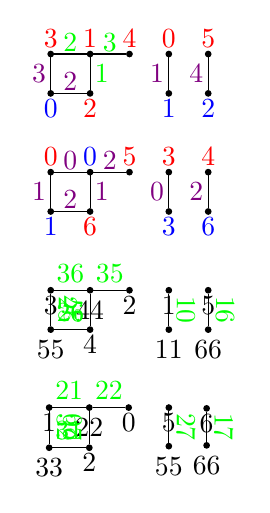
\begin{tikzpicture}[every node/.style={draw, circle, fill=black, minimum size=2pt, inner sep=0pt}]
\node[fill=black, label=below:{\color{blue}$0$}] (G1N0) at (4,7) {};
\node[fill=black, label=below:{\color{red}$2$}] (G1N2) at (4.5,7) {};
\node[fill=black, label=above:{\color{red}$1$}] (G1N1) at (4.5,7.5) {};
\node[fill=black, label=above:{\color{red}$4$}] (G1N4) at (5,7.5) {};
\node[fill=black, label=above:{\color{red}$3$}] (G1N3) at (4,7.5) {};
\node[fill=black, label=above:{\color{red}$0$}] (G1N10) at (5.5,7.5) {};
\node[fill=black, label=below:{\color{blue}$1$}] (G1N11) at (5.5,7) {};
\node[fill=black, label=above:{\color{red}$5$}] (G1N66) at (6,7.5) {};
\node[fill=black, label=below:{\color{blue}$2$}] (G1N22) at (6,7) {};
\draw (G1N2) -- node[midway, right, draw=none, fill=none] {\textcolor{green}{1}} (G1N1);
\draw (G1N2) -- node[midway, sloped, above, draw=none, fill=none] {\textcolor{violet}{2}} (G1N0);
\draw (G1N1) -- node[midway, sloped, above, draw=none, fill=none] {\textcolor{green}{2}} (G1N3);
\draw (G1N1) -- node[midway, sloped, above, draw=none, fill=none] {\textcolor{green}{3}} (G1N4);
\draw (G1N3) -- node[midway, left, draw=none, fill=none] {\textcolor{violet}{3}} (G1N0);
\draw (G1N11) -- node[midway, left, draw=none, fill=none] {\textcolor{violet}{1}} (G1N10);
\draw (G1N22) -- node[midway, left, draw=none, fill=none] {\textcolor{violet}{4}} (G1N66);

%graph 2
\node[fill=black, label=below:{\color{blue}$1$}] (G2N11) at (4,5.5) {};
\node[fill=black, label=below:{\color{red}$6$}] (G2N0) at (4.5,5.5) {};
\node[fill=black, label=above:{\color{blue}$0$}] (G2N10) at (4.5,6) {};
\node[fill=black, label=above:{\color{red}$5$}] (G2N5) at (5,6) {};
\node[fill=black, label=above:{\color{red}$0$}] (G2N6) at (4,6) {};
\node[fill=black, label=below:{\color{blue}$3$}] (G2N33) at (5.5,5.5) {};
\node[fill=black, label=above:{\color{red}$3$}] (G2N3) at (5.5,6) {};
\node[fill=black, label=below:{\color{blue}$6$}] (G2N66) at (6,5.5) {};
\node[fill=black, label=above:{\color{red}$4$}] (G2N4) at (6,6) {};
\draw (G2N0) -- node[midway, right, draw=none, fill=none] {\textcolor{violet}{1}} (G2N10);
\draw (G2N0) -- node[midway, above, draw=none, fill=none] {\textcolor{violet}{2}} (G2N11);
\draw (G2N10) -- node[midway, sloped, above, draw=none, fill=none] {\textcolor{violet}{0}} (G2N6);
\draw (G2N10) -- node[midway, above, draw=none, fill=none] {\textcolor{violet}{2}} (G2N5);
\draw (G2N6) -- node[midway, left, draw=none, fill=none] {\textcolor{violet}{1}} (G2N11);
\draw (G2N3) -- node[midway, left, draw=none, fill=none] {\textcolor{violet}{0}} (G2N33);
\draw (G2N4) -- node[midway, left, draw=none, fill=none] {\textcolor{violet}{2}} (G2N66);
%graph 3
\node[fill=black, label=below:{\color{black}$55$}] (G3N55) at (4,4) {};
\node[fill=black, label=below:{\color{black}$4$}] (G3N4) at (4.5,4) {};
\node[fill=black, label=below:{\color{black}$44$}] (G3N44) at (4.5,4.5) {};
\node[fill=black, label=below:{\color{black}$2$}] (G3N2) at (5,4.5) {};
\node[fill=black, label=below:{\color{black}$3$}] (G3N3) at (4,4.5) {};
\node[fill=black, label=below:{\color{black}$1$}] (G3N1) at (5.5,4.5) {};
\node[fill=black, label=below:{\color{black}$11$}] (G3N11) at (5.5,4) {};
\node[fill=black, label=below:{\color{black}$66$}] (G3N66) at (6,4) {};
\node[fill=black, label=below:{\color{black}$5$}] (G3N5) at (6,4.5) {};
\draw (G3N4) -- node[midway, sloped, above, draw=none, fill=none] {\textcolor{green}{37}} (G3N44);
\draw (G3N4) -- node[midway, sloped, above, draw=none, fill=none] {\textcolor{green}{26}} (G3N55);
\draw (G3N44) -- node[midway, sloped, above, draw=none, fill=none] {\textcolor{green}{36}} (G3N3);
\draw (G3N44) -- node[midway, sloped, above, draw=none, fill=none] {\textcolor{green}{35}} (G3N2);
\draw (G3N3) -- node[midway, sloped, above, draw=none, fill=none] {\textcolor{green}{25}} (G3N55);
\draw (G3N1) -- node[midway, sloped, above, draw=none, fill=none] {\textcolor{green}{10}} (G3N11);
\draw (G3N5) -- node[midway, sloped, above, draw=none, fill=none] {\textcolor{green}{16}} (G3N66);

\node[fill=black, label=below:{\color{black}$33$}] (G4N33) at (3.98,2.50) {};
\node[fill=black, label=below:{\color{black}$2$}] (G4N2) at (4.49,2.50) {};
\node[fill=black, label=below:{\color{black}$22$}] (G4N22) at (4.49,3.01) {};
\node[fill=black, label=below:{\color{black}$0$}] (G4N0) at (4.99,3.01) {};
\node[fill=black, label=below:{\color{black}$1$}] (G4N1) at (3.98,3.01) {};
\node[fill=black, label=below:{\color{black}$5$}] (G4N5) at (5.50,3.01) {};
\node[fill=black, label=below:{\color{black}$55$}] (G4N55) at (5.50,2.52) {};
\node[fill=black, label=below:{\color{black}$66$}] (G4N66) at (5.98,2.53) {};
\node[fill=black, label=below:{\color{black}$6$}] (G4N6) at (5.98,3.00) {};
\draw (G4N2) -- node[midway, sloped, above, draw=none, fill=none] {\textcolor{green}{20}} (G4N22);
\draw (G4N2) -- node[midway, sloped, above, draw=none, fill=none] {\textcolor{green}{31}} (G4N33);
\draw (G4N22) -- node[midway, sloped, above, draw=none, fill=none] {\textcolor{green}{21}} (G4N1);
\draw (G4N22) -- node[midway, sloped, above, draw=none, fill=none] {\textcolor{green}{22}} (G4N0);
\draw (G4N1) -- node[midway, sloped, above, draw=none, fill=none] {\textcolor{green}{32}} (G4N33);
\draw (G4N5) -- node[midway, sloped, above, draw=none, fill=none] {\textcolor{green}{27}} (G4N55);
\draw (G4N6) -- node[midway, sloped, above, draw=none, fill=none] {\textcolor{green}{17}} (G4N66);
\end{tikzpicture}
\end{document}
